\documentclass{standalone}
\usepackage{tikz,pgfplots,calc}
\usetikzlibrary{positioning,calc}
\usetikzlibrary{arrows}
\usepackage{tkz-euclide}
\usetkzobj{all}

\tikzset{
  mynode/.style = {align = center}}

\begin{document}
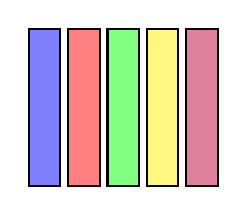
\begin{tikzpicture}[>=stealth', thick]


    % % \node (p0) at (-2, 0) {};
    % % \node [anchor = west, right = 2cm of p0] (p1) {$p_1$};
    % % % \node [anchor = east, left = 2cm of p1.west] (p0) {};
    % % \node [anchor = south east, above left = 1cm and 1cm of p0.north west, blue] (p3) {$p_2$};
    % % \node [anchor = north east, below left = 1cm and 1cm of p0.south west, blue] (p2) {$p_3$};
    % % \node [anchor = north, below = 1cm of p0.south] (p4) {};

    % % \draw [->] (p0) -- (p1);
    % % \draw [->, blue] (p2) -- (p0);
    % % \draw [->, blue] (p3) -- (p0);
    % % \draw [dashed, very thick, violet] (p4) -- (p0);
    % % \node [scale = 1.5, red] at (-5,0) {$C_{12}$};
    % % \node [scale = 1.5, red] at (-5,-5) {$C_{22}$};
    % % \node [scale = 1.5, red] at (-5,-10) {$C_{31}$};
    % % %% ==============================================================
    % % \node (p0) at (5, 0) {};
    % % \node [anchor = east, left = 2cm of p0, blue] (p1) {$p_1$};
    % % % \node [anchor = west, right = 2cm of p1.east] (p0) {};
    % % \node [anchor = south west, above right = 1cm and 1cm of p0.north east] (p2) {$p_2$};
    % % \node [anchor = north west, below right = 1cm and 1cm of p0.south east] (p3) {$p_3$};
    % % \node [anchor = north, below = 1cm of p0.south] (p4) {};

    % % \draw [->, blue] (p1) -- (p0);
    % % \draw [->] (p0) -- (p2);
    % % \draw [->] (p0) -- (p3);
    % % \draw [dashed, violet, very thick] (p4) -- (p0);
    % % %% ==============================================================
    % % \node (p0) at (1, -5) {};
    % % \node [anchor = south east, above left = 1cm and 2.5cm of p0, blue] (p1) {$p_1$};
    % % \node [anchor = north east, below left = 1cm and 2.5cm of p0, blue] (p2) {$p_2$};
    % % \node [anchor = south west, above right = 1.5cm and 2.5cm of p0] (p3) {$p_3$};
    % % \node [anchor = north west, below right = 1.5cm and 2.5cm of p0] (p4) {$p_4$};
    % % \draw [->,blue] (p1) -- (p0);
    % % \draw [->,blue] (p2) -- (p0);
    % % \draw [<-] (p3) -- (p0);
    % % \draw [<-] (p4) -- (p0);
    % % %% ==============================================================
    % % \node (p0) at (-2, -10) {};
    % % \node (p1) [blue,anchor = east, left= 1.5cm of p0] {$p_1$};
    % % \node (p2) [anchor = south west, above right = 1.5cm and 1.5cm of p0] {$p_2$};
    % % \node (p3) [anchor = west, right= 1.5cm of p0] {$p_3$};
    % % \node (p4) [anchor = north west, below right = 1.5cm and 1.5cm of p0] {$p_4$};
    % % \draw [->, blue] (p1) -- (p0);
    % % \draw [->] (p0) -- (p2);
    % % \draw [->] (p0) -- (p3);
    % % \draw [->] (p0) -- (p4);
    % % %% ==============================================================
    % % \node (p0) at (5, -10) {};
    % % \node (p1) [anchor = west, right= 1.5cm of p0] {$p_1$};
    % % \node (p2) [blue,anchor = south east, above left = 1.5cm and 1.5cm of p0] {$p_2$};
    % % \node (p3) [blue,anchor = east, left= 1.5cm of p0] {$p_3$};
    % % \node (p4) [blue,anchor = north east, below left = 1.5cm and 1.5cm of p0] {$p_4$};
    % % \draw [<-] (p1) -- (p0);
    % % \draw [<-, blue] (p0) -- (p2);
    % % \draw [<-, blue] (p0) -- (p3);
    % % \draw [<-, blue] (p0) -- (p4);

    % \def\xx{.5}
    % \def\xy{3}
    % \def\yx{5}
    % \def\yy{1}
    % \coordinate (p0) at (0, 0) {};
    % \coordinate (x) at (\xx, \xy);
    % \coordinate (y) at (\yx, \yy);


    % % \tkzDefPoint[label = above:$x$] (\xx, \xy) {x}
    % % \tkzDefPoint[label = above:$y$] (\yx, \yy) {y}
    % % \tkzDrawPoints[fill=black, size = 1.5] (x,y)
    % % \tkzLabelPoints[above](x, y)
    % \coordinate (xy) at (\xx, \yy);
    % \draw [->] (-.5, 0) --++ (7, 0);
    % \draw [->] (0, -.5) --++ (0, 5);


    % \draw [dashed] (xy) --(\xx, 0);
    % \draw [dashed] (x) --++(-\xx, 0);
    % \node at (\xx, \xy + .2) {$\mathbf{x}$};
    % \node at (\yx, \yy + .2) {$\mathbf{y}$};
    % \node at (\xx + .2, \yy - .2) {$\mathbf{z}$};
    % \node at (\xx, -.25) {$x_1$};
    % \node at (\yx, -.25) {$y_1$};
    % \node at (-.25, \xy) {$x_2$};
    % \node at (-.25, \yy) {$y_2$};
    % \node [rotate = -23] at (.5*\xx + .5*\yx, .5*\xy + .5*\yy + .3) {\textcolor{blue}{$\mathbf{\|\mathbf{x - y}\|_2}$}};
    % \draw [dashed] (y) --(\yx, 0);
    % \draw [dashed] (xy) --( 0, \yy);
    % \draw [blue, thick] (x) -- (y) ; 
    % \draw [red, thick] (x) -- (xy); 
    % \draw [red, thick] (y) -- (xy); 
    % \node at (.5*\xx + .5*\yx, \yy + .3) {\textcolor{red}{${|x_1 - y_1|}$}};
    % \node [rotate = -90, blue] at (\xx+.3, .5*\xy + .5*\yy) {\textcolor{red}{$|x_2 - y_2|$}};
    % \node [red] at (.5*\xx + .5*\yx, .5*\xy + .5*\yy + 1.7) {\textcolor{red}{$\mathbf{\|\mathbf{x - y}\|_1 = |x_1 - y_1| + |x_2 - y_2|}$}};
    % % \draw 
    % % \draw 


% \node [text width = 4cm, align = center] at (0, 0) {Raw training data \\ (both input, output)};
\draw [draw, fill = blue!50] (0, 0) rectangle (.4, 2);
\draw [draw, fill = red!50] (.5, 0) rectangle (.9, 2);
\draw [draw, fill = green!50] (1, 0) rectangle (1.4, 2);
\draw [draw, fill = yellow!50] (1.5, 0) rectangle (1.9, 2);
\draw [draw, fill = purple!50] (2, 0) rectangle (2.4, 2);
\end{tikzpicture}
\end{document}